\documentclass[main.tex]{subfiles} 

\begin{document}
\section*{Analyse}
\label{sec:2}
Hvordan ble undervisningen lagt opp for å skape god begrepsforståelse i naturfagstimene?

Lærer starter dialog, m.a.o lærer tar initiativ(I), elev responderer(R) og responsen blir
evaluert(E) og/eller kommentert(F) av læreren. Ifølge \citeA{klet13} dominerer IRE/F 
metoden klasseromsinteraksjonen. Til den første timen rekker elevene opp hånda for å 
respondere. Det viser seg at det er noen få elever, som viser trygghet og kontroll når 
de responderer til lærer initiert dialog. 

Ved å være bevisst på at alle elevene skal ha kjennskap til 
begrepene som blir tatt opp og repetert, er det da nødvendig å få bekreftet at elevene innehar en 
overordnet forståelse. Det kan derfor være nødvendig å utpeke noen elever som ikke viser aktiv 
deltagelse i timen og frembringe deres respons. Hvis elevene ikke klarer å respondere på lærer 
initiativ, kan utspørringen av elevene vise hull i deres kunnskap. I 2. timen ble denne formen for
utspørringen anvendt til å frembringe respons. 



\citeA[s. ~136]{klet13} beskriver en god undervisningseksens hvor lærere klarer å balansere mellom tilegnelses-,
utprøvings-, og konsolideringssituasjoner. Ifølge Klette har norske klasserom ensidige tendenser i bruken av 
variert arbeidsmåter. Slik det kan ses fra figur \ref{fig:odeg10}, er det for eksempel lite konsolideringssituasjoner.
Lærernes metalæringsaktiviteter regnes som særlig avgjørende for å sikre elevenes læring (\citeNP[s. 186]{klet13}).
Gjennom alle timene har aktivering av forkunnskaper, gjennom repitisjon og gjenbruk av begreper og gjennomgang av 
lekser, bruk av appetittvekker, som i vår tilfellet kan være bruken av en anatomisk modell og observasjon av
encellede organismer gjennom et mikroskop, og tilslutt oppsummering av timen med gjentagelse av prosessen
for flercellede organismer i motsatt rekkefølge, fra organismer med organsystemmer til encellede organismer, har 
alle timene bæret preg av bevisst fokus på bruk av konsolideringssituasjoner/metalæringsaktiviteter. 

Fra figuren kan vi også se at i PIS+ studie i en vanlig naturfagstime brukes mye tid på å utvikle nytt fagstoff.


\begin{figure}[h!]
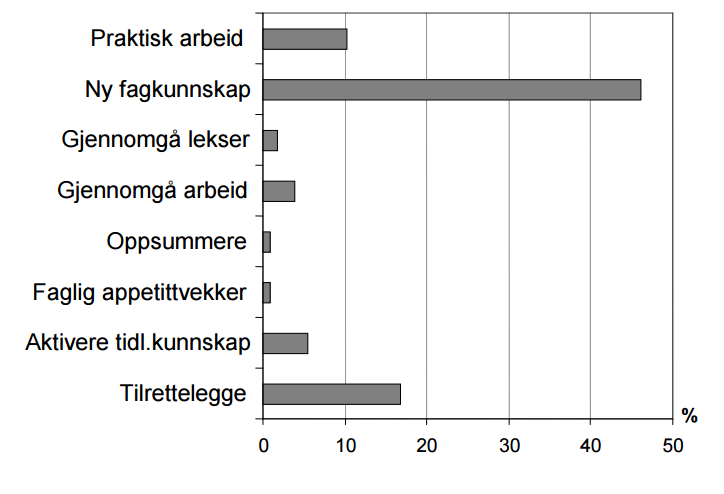
\includegraphics[scale = 0.6]{../figures/undervisnings_aktivitet.png}
\caption{Oversikt over naturfaglærernes undervisningstilbud til elevene fra PISA+ studie. Kilde: \protect\citeA{odeg10}.}
\label{fig:odeg10}
\end{figure}

gode fagsentrerte samtaler mellom elever hvor elever brukte egne erfaringer
og språket for å oppnå faglig forståelse, eller faglige samtaler med lærer som hjelper til å skape
bro mellom praksis og teori 
\citeA{odeg10}


%  ”inquiry-based science teaching” 
\citeA{knai11}

Siden resterende del av timen skal brukes til repetisjon, er det ikke nødvendig å 
prøve å finne svakheter i elevenes respons gjennom helklassesamtalen. For å finne slike svakheter 
ble gruppesamtalene en bedre plattform. I den forbindelse ble tokolonnenotatet tatt i bruk (se 
vedlegg : \ref{sec:tokolonnenotat}).

Timen 2. starter på tilsvarende vis som den første timen. Derimot i denne timen er oppsettet 
forskjellig. Hensikten med timen er å repetere leksene elevene har fått til timen, om celletyper og
utvikling av celler fra enkeltceller til flercelledeorganismer. Etter å konsultert med veilederen
var jeg nå klar over at alle elevene hadde forutsetning til å kunne respondere til våre spørsmål, 
så lenge de var relatert til leksene. Etter den første timen var jeg nå bevisst på at elevenes 
respons var avhengig av deres trygghet med et gitt tema. 

Evnen til abstrahering henger ifølge Vygotsky (\citeNP[s. 127]{bta98}) med begrepsundervisning, som en
form for vitenskapeliggjøring av hverdagsbegreper. Hvis elever ikke har god begrepsforståelse
kan de ende opp med å bruke naturvitenskapelige begreper i feil kontekst og danne feil 
forbindelser med begrepene. Dette avhenger av deres forkunnskaper. Ausubels kognitive bruer 
(\citeNP[s. 71]{math15}), hans teori om begrepslæring på høyere nivå og hvordan læreren best kan legge 
til rette for slik læring og bruk av begrepene,  handler om å danne forbindelser mellom undervisningsmateriell
og relevante ideer i elevenes kognitive struktur.




Til den siste timen hadde vi innsamlet prøver fra en utflukt og lagret de i laboratoriet. 
Gjennom tilstrekkelige forhold hadde vi klart å vokse fram encellede organismer, deriblant tøffeldyr 
(en organisme som er oppkalt etter sko fordi dens utseende ligner på tøfler).

Et premiss for dybdelæring er at elevene får anvendt kunnskapen, og dermed opplever de større grad av faglig utvikling, \citeA{beer14}.


\end{document}
